\section{Modelos de inventario}

\begin{frame}{Simulación de un modelo de inventarios}
    \begin{itemize}
        \item Los estados del sistema se refieren al nivel de inventario actual, pedidos pendientes, existencia de \textit{backorders}.
        \item Los eventos que pueden ocurrir se relacionan con la demanda de unidades del inventario, la revisión de la posición del inventario y la decisión resultante de hacer una orden y la llegada de un pedido.
    \end{itemize}
\end{frame}

\begin{frame}{Sistema de inventarios $(s,S)$}
    \begin{itemize}
        \item Una política de inventarios $(s,S)$, es un sistema de revisión continua.
        \item Si el inventario se encuentra en un nivel igual o menor que $s$ se solicitan suficientes unidades para llevar el inventario a un nivel $S$.
        \item El \textit{lead time}, $l$, puede ser variable.
        \item La demanda por lo general no se conoce con certeza, por lo que puede modelarse a través de una variable aleatoria.
        \item Puede o no admitirse la ocurrencia de \textit{backorders}.
    \end{itemize}
\end{frame}

\begin{frame}{Sistema de inventarios $(s,S)$}
    \begin{figure}
        \centering
        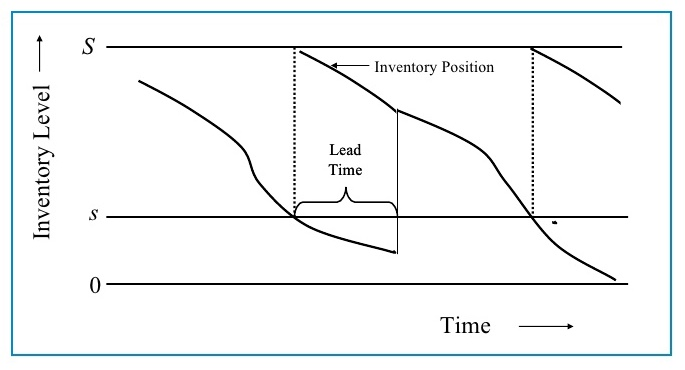
\includegraphics[width=10cm]{images/inventory-management12248440536560389-73-728-2.jpg}
        %\caption{Caption}
        \label{fig:my_label}
    \end{figure}
\end{frame}

\begin{frame}{Parámetros de interés}
    \begin{itemize}
        \item Las políticas de inventario tienen varios parámetros, algunos controlables y otros no.
        \item Entre los parámetros controlables se encuentran:
        \begin{itemize}
            \item Inventario máximo, $S$.
            \item Inventario de seguridad, $s$.
            \item Lead time, $l$.
            \item Periodo de revisión, $t$.
        \end{itemize}
    \end{itemize}
\end{frame}

\begin{frame}{Tabla de simulación para un modelo de inventarios}{}

{\footnotesize
\begin{table}[]
\begin{tabular}{|l|c|c|c|c|c|c|}
\hline
\rowcolor[HTML]{794033} 
{\color[HTML]{FFFFFF} \begin{tabular}[c]{@{}l@{}}Día\\ (rlj)\end{tabular}} &  \multicolumn{1}{l|}{\cellcolor[HTML]{794033}{\color[HTML]{FFFFFF} \begin{tabular}[c]{@{}l@{}}Inv. \\ inicial\\ (estado)\end{tabular}}} & \multicolumn{1}{l|}{\cellcolor[HTML]{794033}{\color[HTML]{FFFFFF} \begin{tabular}[c]{@{}l@{}}Demanda\\ (entrada)\end{tabular}}} & \multicolumn{1}{l|}{\cellcolor[HTML]{794033}{\color[HTML]{FFFFFF} \begin{tabular}[c]{@{}l@{}}Inv. \\ final\\ (est.)\end{tabular}}} & \multicolumn{1}{l|}{\cellcolor[HTML]{794033}{\color[HTML]{FFFFFF} \begin{tabular}[c]{@{}l@{}}Faltante\\ (estado)\end{tabular}}} & \multicolumn{1}{l|}{\cellcolor[HTML]{794033}{\color[HTML]{FFFFFF} \begin{tabular}[c]{@{}l@{}}Orden \\ pend.\\ (est.)\end{tabular}}} & \multicolumn{1}{l|}{\cellcolor[HTML]{794033}{\color[HTML]{FFFFFF} \begin{tabular}[c]{@{}l@{}}Días para \\ llegada \\ orden\\ (estado)\end{tabular}}} \\ \hline
\rowcolor[HTML]{F28165} 
{\color[HTML]{FFFFFF} 0} & {\color[HTML]{FFFFFF} -} & {\color[HTML]{FFFFFF} -} & {\color[HTML]{FFFFFF} 3} & {\color[HTML]{FFFFFF} 0} & {\color[HTML]{FFFFFF} 8} & {\color[HTML]{FFFFFF} 2} \\ \hline
\rowcolor[HTML]{F28165} 
{\color[HTML]{FFFFFF} 1} & {\color[HTML]{FFFFFF} 3} & {\color[HTML]{FFFFFF} 2} & {\color[HTML]{FFFFFF} 1} & {\color[HTML]{FFFFFF} 0} & {\color[HTML]{FFFFFF} 8} & {\color[HTML]{FFFFFF} 1} \\ \hline
\rowcolor[HTML]{F28165} 
{\color[HTML]{FFFFFF} 2} & {\color[HTML]{FFFFFF} 1} & {\color[HTML]{FFFFFF} 1} & {\color[HTML]{FFFFFF} 8} & {\color[HTML]{FFFFFF} 0} & {\color[HTML]{FFFFFF} } & {\color[HTML]{FFFFFF} } \\ \hline
\rowcolor[HTML]{F28165} 
{\color[HTML]{FFFFFF} 3} & {\color[HTML]{FFFFFF} 8} & {\color[HTML]{FFFFFF} 2} & {\color[HTML]{FFFFFF} 6} & {\color[HTML]{FFFFFF} 0} & {\color[HTML]{FFFFFF} } & {\color[HTML]{FFFFFF} } \\ \hline
\rowcolor[HTML]{F28165} 
{\color[HTML]{FFFFFF} 4} & {\color[HTML]{FFFFFF} 6} & {\color[HTML]{FFFFFF} 1} & {\color[HTML]{FFFFFF} 5} & {\color[HTML]{FFFFFF} 0} & {\color[HTML]{FFFFFF} } & {\color[HTML]{FFFFFF} } \\ \hline
\rowcolor[HTML]{F28165} 
{\color[HTML]{FFFFFF} 5} & {\color[HTML]{FFFFFF} 5} & {\color[HTML]{FFFFFF} 2} & {\color[HTML]{FFFFFF} 3} & {\color[HTML]{FFFFFF} 0} & {\color[HTML]{FFFFFF} 8} & {\color[HTML]{FFFFFF} 1} \\ \hline
\rowcolor[HTML]{F28165} 
{\color[HTML]{FFFFFF} 6} & {\color[HTML]{FFFFFF} 3} & {\color[HTML]{FFFFFF} 3} & {\color[HTML]{FFFFFF} 8} & {\color[HTML]{FFFFFF} 0} & {\color[HTML]{FFFFFF} } & {\color[HTML]{FFFFFF} } \\ \hline
\rowcolor[HTML]{F28165} 
{\color[HTML]{FFFFFF} 7} & {\color[HTML]{FFFFFF} 8} & {\color[HTML]{FFFFFF} 2} & {\color[HTML]{FFFFFF} 6} & {\color[HTML]{FFFFFF} 0} & {\color[HTML]{FFFFFF} } & {\color[HTML]{FFFFFF} } \\ \hline
\rowcolor[HTML]{F28165} 
{\color[HTML]{FFFFFF} 8} & {\color[HTML]{FFFFFF} 6} & {\color[HTML]{FFFFFF} 3} & {\color[HTML]{FFFFFF} 3} & {\color[HTML]{FFFFFF} 0} & {\color[HTML]{FFFFFF} 8} & {\color[HTML]{FFFFFF} 2} \\ \hline
\rowcolor[HTML]{F28165} 
{\color[HTML]{FFFFFF} 9} & {\color[HTML]{FFFFFF} 3} & {\color[HTML]{FFFFFF} 2} & {\color[HTML]{FFFFFF} 1} & {\color[HTML]{FFFFFF} 0} & {\color[HTML]{FFFFFF} 8} & {\color[HTML]{FFFFFF} 1} \\ \hline
\rowcolor[HTML]{F28165} 
{\color[HTML]{FFFFFF} 10} & {\color[HTML]{FFFFFF} 1} & {\color[HTML]{FFFFFF} 3} & {\color[HTML]{FFFFFF} 6} & {\color[HTML]{FFFFFF} 0} & {\color[HTML]{FFFFFF} } & {\color[HTML]{FFFFFF} } \\ \hline
\end{tabular}
\end{table}}
\end{frame}


\begin{frame}{Medidas de desempeño}
    \begin{itemize}
        \item Algunas medidas de desempeño de interés son:
        \begin{itemize}
            \item Ingresos totales por ventas.
            \item Costos totales de la política de inventario.
            \item Inventario a la mano promedio.
            \item Nivel de backorders promedio.
            \item Ciclo del inventario promedio.
        \end{itemize}
    \end{itemize}
\end{frame}
